\chapter{Experiments \& Results}
We test our methods on a binary classification task
provided by the SST-2 dataset \parencite{sst2}. 
The dataset consists of
sentences and smaller groups of words
extracted from movie reviews and 
human annotations of their sentiment as either 
positive (1) or negative (0). \autoref{table: sst2} 
shows some example input-output pairs. 

As our base model we use DistilBERT \parencite{distilbert},
which is a transformer model that 
uses knowledge distillation to reduce the size of a 
BERT model. The model consists of an embedding layer 
and 6 transformer layers with a hidden size of 768. 
For the binary classification task, a classification head
is attached to the base model, which is a fully-connected
feed-forward network consisting of a hidden layer of 
size 768 with \ac{ReLU} activation 
and an output layer of size 2. For our experiments we 
train only this classification head, which means we 
optimize 4 tensors: 
\begin{equation*}
    \mathbf{W}_1 \in \mathbb{R}^{768\times768};\quad 
    \mathbf{b}_1 \in \mathbb{R}^{1\times768};\quad 
    \mathbf{W}_2 \in \mathbb{R}^{768\times2};\quad 
    \mathbf{b}_2 \in \mathbb{R}^{1\times2}
\end{equation*}
Unless explicitly stated otherwise, we train all 
parameters of $\mathbf{b}_1, \mathbf{W}_2$ and 
$\mathbf{b}_2$, and randomly 
select $768\times2=1536$ parameters 
from $\mathbf{W}_1$ to perturb per iteration. 

Since we train only the classification head and not the
base model, we configure forward passes to calculate 
the output of the base model only once per iteration. 
This output is stored and further forward passes 
required by the algorithm in the same iteration 
calculate only the pass through the classification head,
improving the speed of computation.
% Later, we extend our experiments to use RoBERTa-large
% \parencite{roberta} as the base model. The classification head
% of this larger model has the same two-layer 
% structure but with a hidden size of 1024.  

We use \autoref{algorithm:options} for all experiments.
When an experiment does not involve options, we set 
both the number of option
levels $\ell$ and the number of options per level $m$ 
to 1, making it the equivalent of \autoref{algorithm:main}.
To ensure reproducibility, experiments set all 
random seeds to $42$. 

\begin{table}
    \centering
    \caption{Example input-output pairs from the SST-2 dataset}
    \label{table: sst2}
    \bigskip
    \begin{tabular}{l c}
        \toprule
        \textbf{Sentence} & \textbf{Label} \\
        \midrule
        contains no wit , only labored gags & 0 \\
        with his usual intelligence and subtlety  & 1\\
        we never feel anything for these characters & 0\\
        equals the original and in some ways even betters it & 1 \\
        \bottomrule
    \end{tabular}
\end{table}

\section{Hyperparameters}
There are several hyperparameters that can influence
the performance of \autoref{algorithm:main}. As discussed 
in \autoref{section:partitioning}, we define the search 
interval through a maximal radius $R$ and the number of 
searches per iteration $K$. Both $R$ and $K$ are 
hyperparameters as well as the batch size $b$.
Testing our main algorithm, we are interested in seeing 
how each of those hyperparameters affect performance.

\autoref{figure:r} shows validation 
accuracy for 3 of our experiments with different 
values for the maximal radius $R$
where we use the same $R$ for each of the 4 tensors.
As expected, the maximal radius $R$ is a deciding factor 
for the algorithm's performance. 
Generally, when $R$ is too low improvement is slow.
When it is too high, updates are noisy and the algorithm
fails to converge at a good minimum. 
We decide that $R=5\cdot10^{-3}$ is an adequate 
default value. 

The number of searches per iteration $K$ decides the 
size of the search interval. We expect better performance
with bigger intervals. The results shown in 
\autoref{figure:k} confirm this for 
small $K$. However, there are diminishing returns as 
$K$ grows.
% Conveniently, with only 1 search radius 
% we are able to get reasonable accuracy. 
Conveniently, the run with only one search radius per
iteration is able to get reasonable accuracy on 
our dataset. We remark that this might 
not be representative in general.
We note that for $K=1$, parameter updates behave like a 
stochastic two points update, 
where the algorithm decides whether the parameter should be 
updated with the given perturbation of radius $R$ or not. 
In particular, there is no binary search.

\begin{figure}
    \centering
    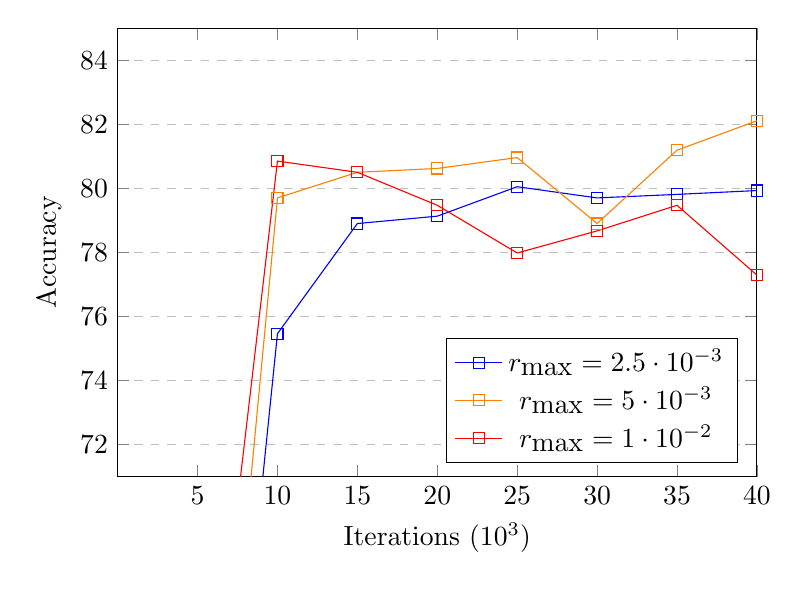
\begin{tikzpicture}
        \begin{axis}[
            width=0.8\textwidth,
            height=\axisdefaultheight,
            xlabel = {Iterations ($10^3$)},
            ylabel = {Accuracy},
            ymin = 71, ymax = 85, 
            xmin = 0, xmax = 40,
            xtick = {5, 10, 15, 20, 25, 30, 35, 40},
            ytick = {72, 74, 76, 78, 80, 82, 84},
            ymajorgrids = true,
            yminorgrids = true,
            legend pos = south east,
            grid style = dashed
        ]
        \addplot[color=blue, mark=square]
            coordinates {(0,0)(5, 51.03)(10,75.46)(15, 78.90)(20, 79.13)(25, 80.05)(30, 79.70)(35, 79.81)(40, 79.93)};
            \addlegendentry{$r_{\textrm{max}} = 2.5\cdot10^{-3}$}
    
        \addplot[color=orange, mark=square]
            coordinates {(0,0)(5, 53.33)(10,79.70)(15,80.50)(20, 80.62)(25, 80.96)(30, 78.90)(35, 81.19)(40, 82.11)};
            \addlegendentry{$r_{\textrm{max}} = 5\cdot10^{-3}$}
        
        \addplot[color=red, mark=square]
            coordinates {(0,0)(5, 59.52)(10,80.85)(15,80.50)(20, 79.47)(25, 77.98)(30, 78.67)(35, 79.47)(40, 77.29)};
            \addlegendentry{$r_{\textrm{max}} = 1\cdot10^{-2}$}    
    
        \end{axis}
    \end{tikzpicture}
    \caption[Validation Accuracy with different maximal search radii]
    {Validation Accuracy for three different values of maximal search radius.  
    $K$ is set to 5, batch size is 64.}
    \label{figure:r}
\end{figure}

\begin{figure}
    \centering
    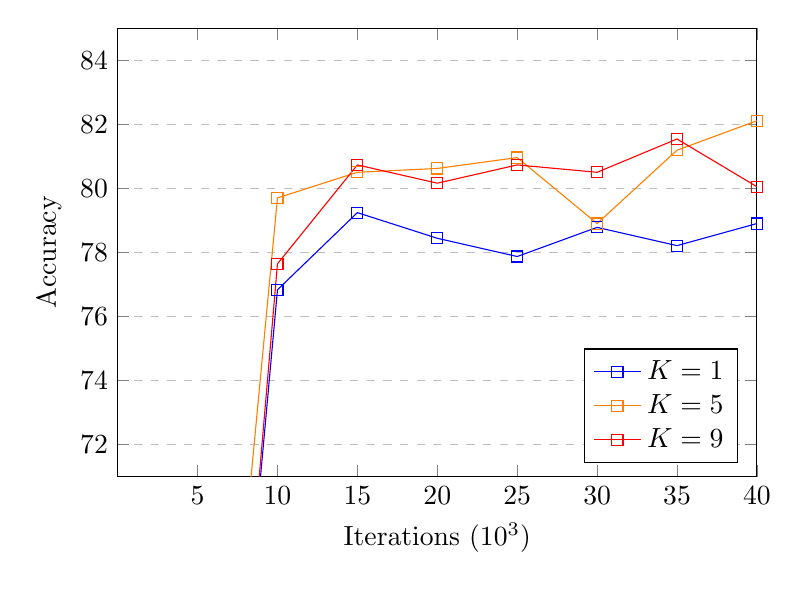
\begin{tikzpicture}
        \begin{axis}[
            width=0.8\textwidth,
            height=\axisdefaultheight,
            xlabel = {Iterations ($10^3$)},
            ylabel = {Accuracy},
            ymin = 71, ymax = 85, 
            xmin = 0, xmax = 40,
            xtick = {5, 10, 15, 20, 25, 30, 35, 40},
            ytick = {72, 74, 76, 78, 80, 82, 84},
            ymajorgrids = true,
            yminorgrids = true,
            legend pos = south east,
            grid style = dashed
        ]
        \addplot[color=blue, mark=square]
            coordinates {(0,0)(5, 49.31)(10,76.83)(15,79.24)(20, 78.44)(25, 77.87)(30, 78.78)(35, 78.21)(40, 78.90)};
            \addlegendentry{$K=1$}
    
        \addplot[color=orange, mark=square]
            coordinates {(0,0)(5, 53.33)(10,79.70)(15,80.50)(20, 80.62)(25, 80.96)(30, 78.90)(35, 81.19)(40, 82.11)};
            \addlegendentry{$K=5$}
    
        \addplot[color=red, mark=square]
            coordinates {(0,0)(5, 48.51)(10,77.64)(15,80.73)(20, 80.16)(25, 80.73)(30, 80.50)(35, 81.54)(40, 80.05)};
            \addlegendentry{$K=9$}
        \end{axis}
    \end{tikzpicture}
    \caption[Validation Accuracy with different number
    of searches]
    {Validation Accuracy when performing
    1, 5 and 9 searches per iteration
    with maximal radius $R=5\cdot10^{-3}$. 
    Batch size is 64.}
    \label{figure:k}
\end{figure}

The batch size $b$ has the most significant effect on 
performance. \autoref{figure:b} shows 
validation accuracy with 3 different batch sizes.
We find that larger batch sizes perform 
consistently better. The drawback is a higher memory 
and time consumption with constant 
step count. We find the results with $b=64$ to be 
adequate and therefore conduct most of our experiments
with a batch size of 64.


\begin{figure}
    \centering
    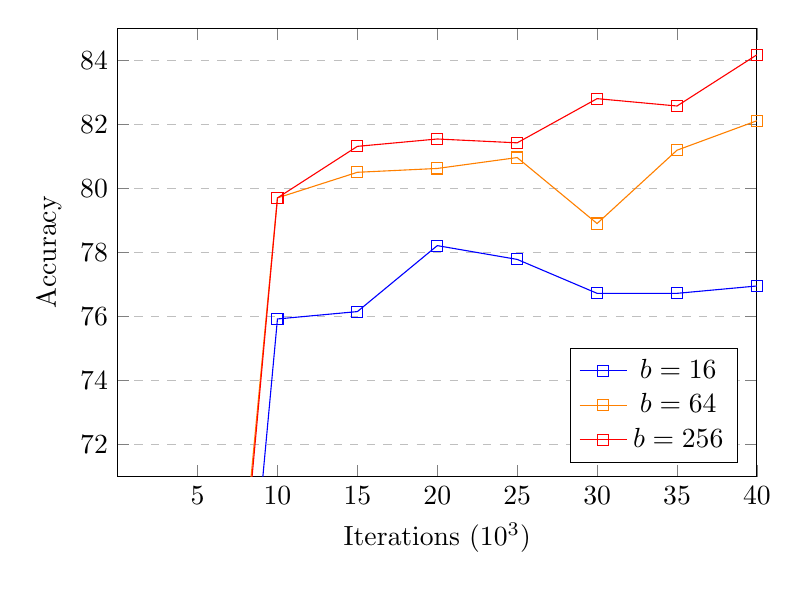
\begin{tikzpicture}
        \begin{axis}[
            width=0.8\textwidth,
            height=\axisdefaultheight,
            xlabel = {Iterations ($10^3$)},
            ylabel = {Accuracy},
            ymin = 71, ymax = 85, 
            xmin = 0, xmax = 40,
            xtick = {5, 10, 15, 20, 25, 30, 35, 40},
            ytick = {72, 74, 76, 78, 80, 82, 84},
            ymajorgrids = true,
            yminorgrids = true,
            legend pos = south east,
            grid style = dashed
        ]
        \addplot[color=blue, mark=square]
            coordinates {(0,0)(5, 48.97)(10,75.92)(15,76.15)(20, 78.21)(25, 77.78)(30, 76.72)(35, 76.72)(40, 76.95)};
            \addlegendentry{$b = 16$}
    
        \addplot[color=orange, mark=square]
            coordinates {(0,0)(5, 53.33)(10,79.70)(15,80.50)(20, 80.62)(25, 80.96)(30, 78.90)(35, 81.19)(40, 82.11)};
            \addlegendentry{$b = 64$}
    
        \addplot[color=red, mark=square]
            coordinates {(0,0)(5, 52.29)(10,79.70)(15,81.31)(20, 81.54)(25, 81.42)(30, 82.80)(35, 82.57)(40, 84.17)};
            \addlegendentry{$b = 256$}
        \end{axis}
    \end{tikzpicture}
    \caption[Validation Accuracy with different batch sizes]
    {Validation Accuracy with 3 different batch sizes.
    $K$ is set to 5, $R$ is set to $5\cdot10^{-3}$.}
    \label{figure:b}
\end{figure}

Since they provide a suitable balance between performance,
memory and time consumption, we decide to take 
$R=5\cdot10^{-3}$, $K = 5$ and $b=64$ as
the set of hyperparameters we use when 
testing our other approaches and modifications over 
the base algorithm. In the following, we refer to this 
configuration as "default hyperparameters". 

% \begin{figure}
%     \centering
%     \begin{tikzpicture}
%         \begin{axis}[
%             width=0.8\textwidth,
%             height=\axisdefaultheight,
%             xlabel = {Iterations ($10^3$)},
%             ylabel = {Accuracy},
%             ymin = 0.35, ymax = 0.75, 
%             xmin = 0, xmax = 40,
%             xtick = {5, 10, 15, 20, 25, 30, 35, 40},
%             ytick = {0.4, 0.45, 0.5, 0.55, 0.6, 0.65, 0.7},
%             ymajorgrids = true,
%             yminorgrids = true,
%             legend pos = north east,
%             grid style = dashed
%         ]
%         \addplot[color=blue, mark=square]
%             coordinates {(0,1)(5, 0.6988)(10,0.5336)(15, 0.4618)(20, 0.4291)(25, 0.4125)(30, 0.404)(35, 0.3965)(40, 0.3897)};
%             \addlegendentry{$R = 2.5\cdot10^{-3}$}
    
%         \addplot[color=orange, mark=square]
%             coordinates {(0,1)(5, 0.7539)(10,0.4548)(15,0.4108)(20, 0.4073)(25, 0.3964)(30, 0.4014)(35, 0.3959)(40, 0.3945)};
%             \addlegendentry{$R = 5\cdot10^{-3}$}
        
%         \addplot[color=red, mark=square]
%             coordinates {(0,1)(5, 1.059)(10,0.4164)(15,0.4193)(20, 0.4304)(25, 0.4524)(30, 0.4569)(35, 0.493)(40, 0.4858)};
%             \addlegendentry{$R = 1\cdot10^{-2}$}    
    
%         \end{axis}
%     \end{tikzpicture}
%     \caption[Validation Accuracy for 3 different values of $R$]
%     {Validation Accuracy for 3 different values of $R$.  
%     $K$ is set to 5, batch size is 64.}
%     \label{figure:rtrain}
% \end{figure}

\section{Parameter Partitioning Methods} \label{section:partition}
In \autoref{section:partitioning}, we introduced 3 methods
to partition tensors that are too large 
to be trained efficiently by \ac{GLD}: We either sample
random indices or rank parameters based on absolute value 
or Fisher information estimate. The absolute value
and Fisher methods aim to select the most important 
parameters to train, improving the convergence rate as
the algorithm does not spend time on training unimportant
parameters with little effect on the outcome. 
From the four tensors we are training, 
% $\mathbf{W}_2, \mathbf{b}_1$ and $\mathbf{b}_2$ 
% have at most $768\times2$ parameters.  
$\mathbf{W}_1$ is the largest with size $768\times768$, 
followed by $\mathbf{W}_1$ with size $768\times2$.
We find that our algorithm can reliably train 
$768\times2$ parameters at a time, but $768\times768$ 
is too large. Therefore, we choose to select and train 
only $768\times2$
parameters from $\mathbf{W}_1$ per iteration. 
\autoref{figure:partition} shows validation loss
when training all parameters of $\mathbf{W}_1$ and when 
selecting $768\times2$ parameters randomly, through 
absolute value and through Fisher information estimate. 
$\mathbf{b}_1, \mathbf{W}_2$ and $\mathbf{b}_2$ each 
train all of their parameters. 
For the Fisher method we get a new Fisher information 
estimate every 10,000 steps. 
The algorithm diverges when training all $768\times768$
parameters of $\mathbf{W}_1$ using the default maximal 
radius. 
We find that contrary to our expectations, the importance 
methods do not bring an improvement on the rate of 
convergence. The performance of the absolute value method is 
comparable to that of the random method while the Fisher method 
performs worse. 
% We surmise that since the random method 
% does not discriminate based on some importance metric, 
% it trains all parameters more consistently, which ends
% up being beneficial for training with the given 
% configuration.

\begin{figure}
    \centering
    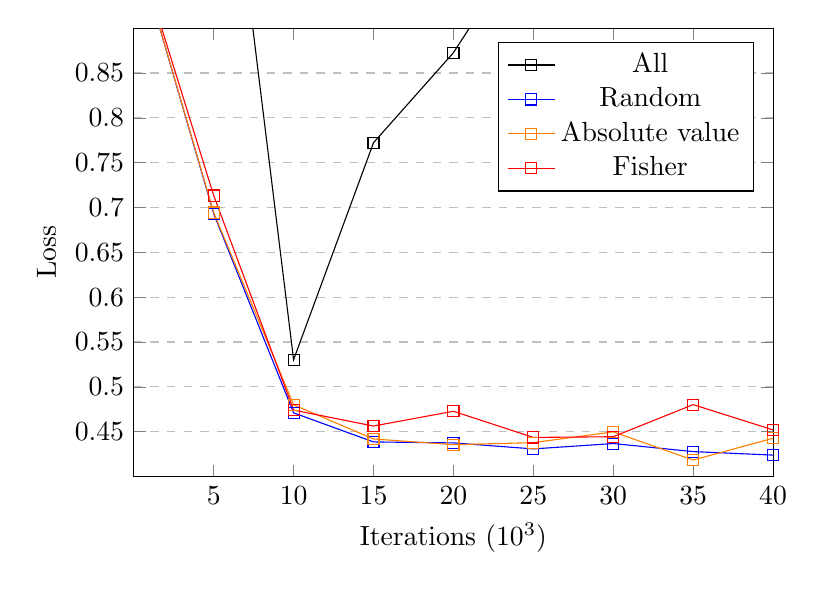
\begin{tikzpicture}
        \begin{axis}[
            width=0.8\textwidth,
            height=\axisdefaultheight,
            xlabel = {Iterations ($10^3$)},
            ylabel = {Loss},
            ymin = 0.40, ymax = 0.9, 
            xmin = 0, xmax = 40,
            xtick = {5, 10, 15, 20, 25, 30, 35, 40},
            ytick = {0.45, 0.50, 0.55, 0.60, 0.65, 0.7, 0.75, 0.8, 0.85},
            ymajorgrids = true,
            yminorgrids = true,
            legend pos = north east,
            grid style = dashed
        ]
        \addplot[color=black, mark=square]
            coordinates {(0,1)(5, 1.255)(10,0.5303)(15,0.7723)(20, 0.8727)(25, 1.01)(30, 1.091)(35, 1.139)(40, 1.388)};
            \addlegendentry{All}

        \addplot[color=blue, mark=square]
            coordinates {(0,1)(5, 0.6932)(10,0.471)(15,0.4386)(20, 0.4375)(25, 0.4308)(30, 0.4368)(35, 0.4278)(40, 0.4239)};
            \addlegendentry{Random}
    
        \addplot[color=orange, mark=square]
            coordinates {(0,1)(5, 0.6944)(10,0.4800)(15,0.4419)(20, 0.4355)(25, 0.4378)(30, 0.4498)(35, 0.4184)(40, 0.4427)};
            \addlegendentry{Absolute value}
    
        \addplot[color=red, mark=square]
            coordinates {(0,1)(5, 0.7134)(10,0.4741)(15,0.4563)(20, 0.4728)(25, 0.4436)(30, 0.4444)(35, 0.4802)(40, 0.4520)};
            \addlegendentry{Fisher}
        \end{axis}
    \end{tikzpicture}
    \caption[Validation loss with different parameter partitioning methods]
    {Validation loss of different parameter partitioning methods on 
    $\mathbf{W}_1$ using default hyperparameters. Other tensors are not split.}
    \label{figure:partition}
\end{figure}

% \begin{figure}
%     \centering
%     \begin{tikzpicture}
%         \begin{axis}[
%             width=0.8\textwidth,
%             height=\axisdefaultheight,
%             xlabel = {Iterations ($10^3$)},
%             ylabel = {Accuracy},
%             ymin = 71, ymax = 85, 
%             xmin = 0, xmax = 40,
%             xtick = {5, 10, 15, 20, 25, 30, 35, 40},
%             ytick = {72, 74, 76, 78, 80, 82, 84},
%             ymajorgrids = true,
%             yminorgrids = true,
%             legend pos = south east,
%             grid style = dashed
%         ]
%         \addplot[color=blue, mark=square]
%             coordinates {(0,0)(5, 51.72)(10,78.9)(15,80.05)(20, 80.50)(25, 79.7)(30, 79.7)(35, 81.08)(40, 79.82)};
%             \addlegendentry{Absolute value}
    
%         \addplot[color=orange, mark=square]
%             coordinates {(0,0)(5, 53.33)(10,79.70)(15,80.50)(20, 80.62)(25, 80.96)(30, 78.90)(35, 81.19)(40, 82.11)};
%             \addlegendentry{Random}
    
%         \addplot[color=red, mark=square]
%             coordinates {(0,0)(5, 50.92)(10,78.9)(15,79.24)(20, 78.33)(25, 78.33)(30, 79.36)(35, 75.23)(40, 78.67)};
%             \addlegendentry{Fisher}
%         \end{axis}
%     \end{tikzpicture}
%     \caption[Partition]
%     {Partition}
%     \label{figure:partitionacc}
% \end{figure}

\section{Radius Scheduling} \label{section:schedule}
We introduce a radius scheduler to each of the trainable 
tensors that reduces the maximum search radius 
as training goes on. We use a linear schedule $s$ that scales 
from 1 to $h = 0.1$ over the course of training $T$ steps:
\begin{equation}
    s(t) = 1 - \frac{t(1-h)}{T}                                                                                                                                                                                                                                                                                                                                                                                                                                                                                                                                                                                                                                                                                                                                                                                                                                                                                                                                                                                                                                                                                                                                                                                                                                                                                                                                                                                                                                                                                                                                                                                                                                                                                                                                                                                                                                                                                                                                                                                                                                                                                                                                                                                                                                                                                                                                                                                                                                                             
\end{equation}
Maximal radius at step $t$ is calculated by 
multiplying the 
maximal radius of the tensor with the schedule:
\begin{equation}
    R(\bm{\theta}_t) = R(\bm{\theta}) \cdot s(t)
\end{equation}
We use the same schedule with all parameters as well as 
the same initial maximal radius. \autoref{figure:schedule}
shows the validation loss for this experiment in comparison
to the original result with no schedule. 
We find that 
without the radius schedule the model learns faster 
initially but overall loss is less stable and 
the radius scheduler outperforms at later steps. 
Still, a confident increase in performance is not 
observed with default hyperparameters. 
One of our hypotheses was that using a radius scheduler,
the algorithm could retain its convergence with 
fewer searches. To test this, 
We redo the experiment with $K=1$. The results are shown in 
\autoref{figure:schedule2}.
We observe that the effect of the radius scheduler 
is amplified when doing only one search per iteration.
In particular, it causes loss to more consistently decrease 
throughout the entire duration of training. 
While $K=5$ still performs better, the gap is significantly
smaller. We surmise that a smaller $K$ could be used in 
conjunction with a radius scheduler when an increase in 
computation speed is desired.


\begin{figure}
    \centering
    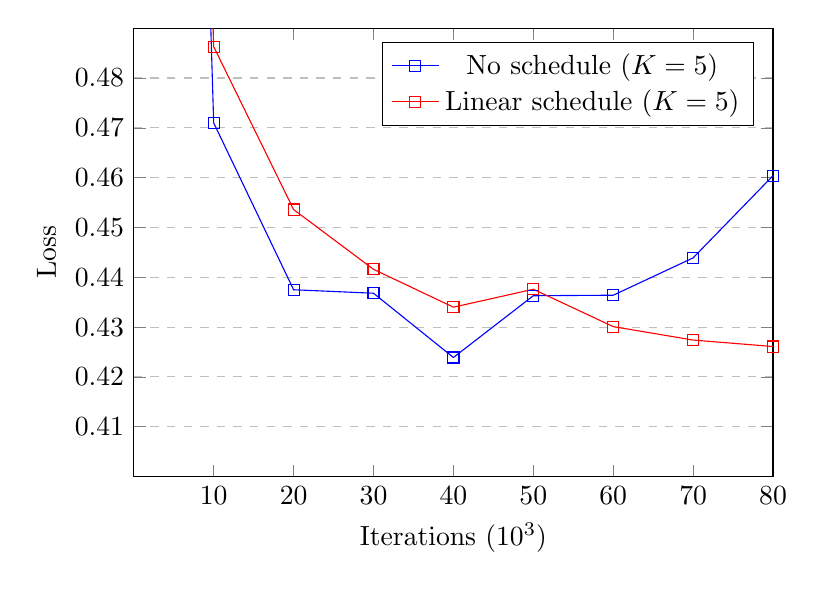
\begin{tikzpicture}
        \begin{axis}[
            width=0.8\textwidth,
            height=\axisdefaultheight,
            xlabel = {Iterations ($10^3$)},
            ylabel = {Loss},
            ymin = 0.40, ymax = 0.49, 
            xmin = 0, xmax = 80,
            xtick = {10, 20, 30, 40, 50, 60, 70, 80},
            ytick = {0.41, 0.42, 0.43, 0.44, 0.45, 0.46, 0.47, 0.48},
            ymajorgrids = true,
            yminorgrids = true,
            legend pos = north east,
            grid style = dashed
        ]
        \addplot[color=blue, mark=square]
            coordinates {(0,1)(10,0.471)(20, 0.4375)(30, 0.4368)(40, 0.4239)(50, 0.4363)(60, 0.4364)(70, 0.4439)(80, 0.4604)};
            \addlegendentry{No schedule ($K=5$)}
    
        \addplot[color=red, mark=square]
            coordinates {(0,1)(10,0.4863)(20, 0.4536)(30, 0.4416)(40,0.434)(50,0.4376)(60,0.4301)(70, 0.4274)(80, 0.4261)};
            \addlegendentry{Linear schedule ($K=5$)}
        \end{axis}
    \end{tikzpicture}
    \caption[Validation loss with and without a radius scheduler]
    {Validation loss with and without a linear radius 
    scheduler using default hyperparameters}
    \label{figure:schedule}
\end{figure}

\begin{figure}
    \centering
    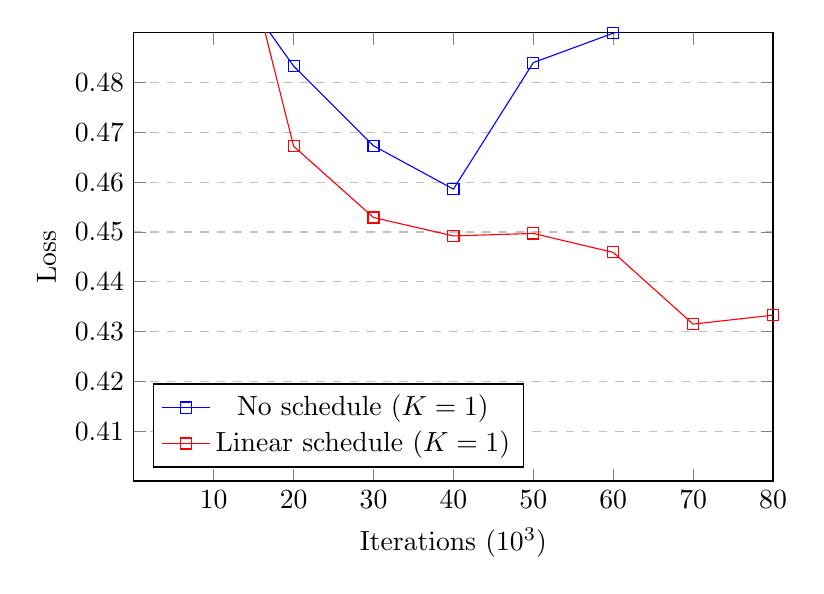
\begin{tikzpicture}
        \begin{axis}[
            width=0.8\textwidth,
            height=\axisdefaultheight,
            xlabel = {Iterations ($10^3$)},
            ylabel = {Loss},
            ymin = 0.40, ymax = 0.49, 
            xmin = 0, xmax = 80,
            xtick = {10, 20, 30, 40, 50, 60, 70, 80},
            ytick = {0.41, 0.42, 0.43, 0.44, 0.45, 0.46, 0.47, 0.48},
            ymajorgrids = true,
            yminorgrids = true,
            legend pos = south west,
            grid style = dashed
        ]
        \addplot[color=blue, mark=square]
            coordinates {(0,1)(10, 0.5058)
            (20,0.4833)(30,0.4673)
            (40, 0.4586)(50, 0.484)
            (60, 0.4899)(70, 0.495)
            (80, 0.4924)};
            \addlegendentry{No schedule ($K=1$)}

        \addplot[color=red, mark=square]
            coordinates {(0,1)
            (10,0.5313)
            (20, 0.4672)
            (30, 0.4529)
            (40,0.4492)
            (50,0.4497)
            (60,0.4459)
            (70, 0.4315)
            (80, 0.4333)};
            \addlegendentry{Linear schedule ($K=1$)}
        \end{axis}
    \end{tikzpicture}
    \caption[Validation loss with and without a radius scheduler with only one search per iteration]
    {Validation loss with and without a linear radius 
    scheduler when performing only one search per iteration}
    \label{figure:schedule2}
\end{figure}

\section{Weight Decay}
We investigate the effects of adding an $L_2$-regularizer 
to the objective function:
\begin{equation}
    \mathcal{J}(\bm{\theta}) = \mathcal{L}(\bm{\theta}) + \lambda \cdot \Vert \bm{\theta} \Vert_2
\end{equation}
where $\mathcal{L}$ is the cross-entropy loss and 
$\lambda$ is the norm weight. 
\autoref{figure:decay} compares three different values
of $\lambda$. Our original experiment without weight decay
has $\lambda = 0$. We observe a more stable decrease in 
loss with regularization. The hyperparameter $\lambda$ 
plays a crucial role in the effectiveness of this method 
as it controls the balance between regularization
and error minimization. We consider
$\lambda = 0.05$ to be a good default value. 

\begin{figure}
    \centering
    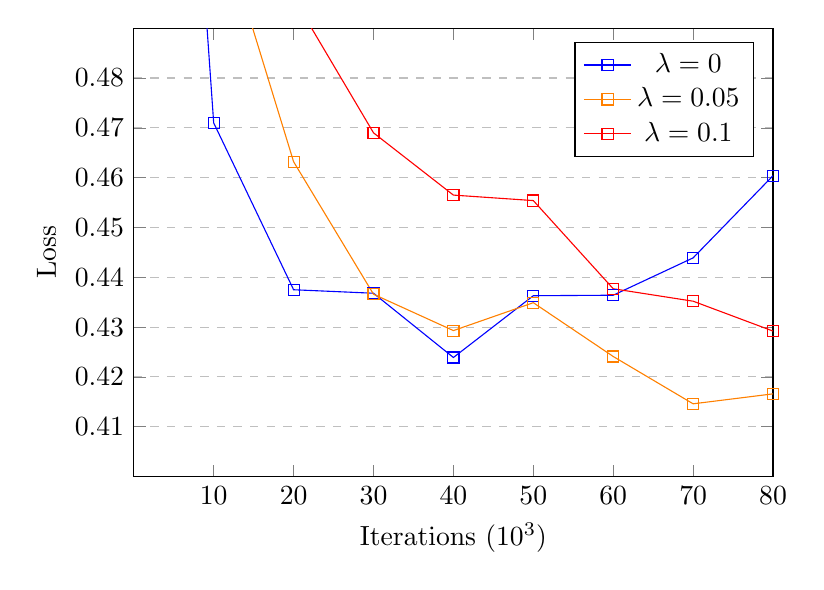
\begin{tikzpicture}
        \begin{axis}[
            width=0.8\textwidth,
            height=\axisdefaultheight,
            xlabel = {Iterations ($10^3$)},
            ylabel = {Loss},
            ymin = 0.40, ymax = 0.49, 
            xmin = 0, xmax = 80,
            xtick = {10, 20, 30, 40, 50, 60, 70, 80},
            ytick = {0.41, 0.42, 0.43, 0.44, 0.45, 0.46, 0.47, 0.48},
            ymajorgrids = true,
            yminorgrids = true,
            legend pos = north east,
            grid style = dashed
        ]
        \addplot[color=blue, mark=square]
            coordinates {(0,0.7)(10,0.471)(20, 0.4375)(30, 0.4368)(40, 0.4239)(50, 0.4363)(60, 0.4364)(70, 0.4439)(80, 0.4604)};
            \addlegendentry{$\lambda = 0$}
    
        \addplot[color=orange, mark=square]
            coordinates {(0,0.7)
            (10, 0.5155)
            (20, 0.4632)
            (30, 0.4366)
            (40, 0.4293)
            (50, 0.4349)
            (60, 0.4241)
            (70, 0.4146)
            (80, 0.4166)};
            \addlegendentry{$\lambda = 0.05$}

        \addplot[color=red, mark=square]
            coordinates {(0,0.7)
            (10, 0.5435)
            (20, 0.4961)
            (30, 0.469)
            (40, 0.4565)
            (50, 0.4554)
            (60, 0.4377)
            (70, 0.4352)
            (80, 0.4292)};
            \addlegendentry{$\lambda = 0.1$}
        \end{axis}
    \end{tikzpicture}
    \caption[Validation loss using weight decay with different norm weights]
    {Validation loss using weight decay with different norm weights.}
    \label{figure:decay}
\end{figure}


\section{Options}
\autoref{algorithm:options} introduces 2 additional 
hyperparameters: The number of option levels $\ell$ and
the number of options per level $m$. Both hyperparameters
have a significant effect on 
the time requirement of the algorithm: The number of 
forward passes each iteration is $n \cdot m^\ell \cdot K$ 
when training $n$ tensors. Therefore, 
although we anticipate a reduction in update noise 
when using options, we have to pick $\ell$ and $m$ 
conservatively in order to keep within a reasonable 
computation time. \autoref{figure:options} shows validation 
loss for four experiments with different values of 
$m$ and $\ell$, each of them named $m \times \ell$.
We observe moderate improvements in loss as $m \times \ell$
increases with $\ell$ having a larger effect than $m$. 

\begin{figure}
    \centering
    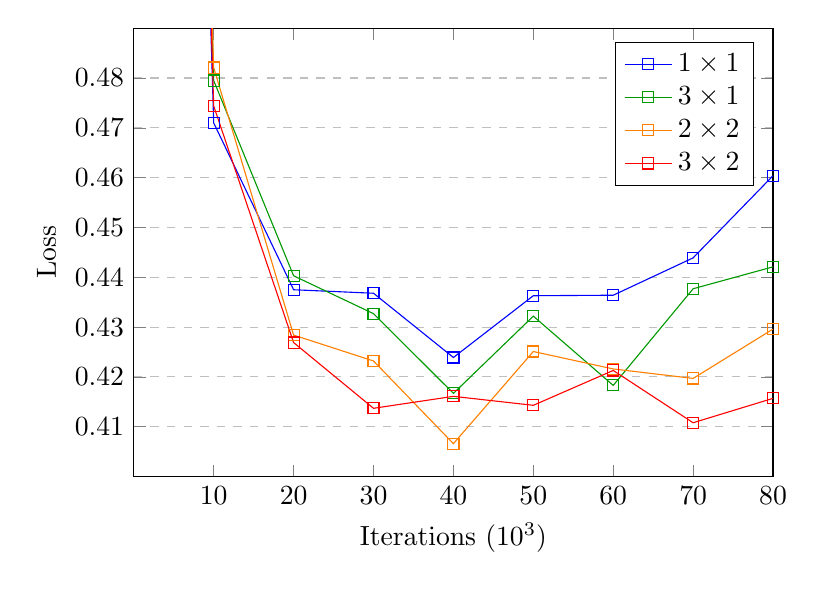
\begin{tikzpicture}
        \begin{axis}[
            width=0.8\textwidth,
            height=\axisdefaultheight,
            xlabel = {Iterations ($10^3$)},
            ylabel = {Loss},
            ymin = 0.40, ymax = 0.49, 
            xmin = 0, xmax = 80,
            xtick = {10, 20, 30, 40, 50, 60, 70, 80},
            ytick = {0.41, 0.42, 0.43, 0.44, 0.45, 0.46, 0.47, 0.48},
            ymajorgrids = true,
            yminorgrids = true,
            legend pos = north east,
            grid style = dashed
        ]
        \addplot[color=blue, mark=square]
            coordinates {(0,1)(10,0.471)(20, 0.4375)(30, 0.4368)(40, 0.4239)(50, 0.4363)(60, 0.4364)(70, 0.4439)(80, 0.4604)};
            \addlegendentry{$1\times1$}

        \addplot[color=green!60!black, mark=square]
            coordinates { (0,1)
            (10, 0.4795)
            (20, 0.4403)
            (30, 0.4327)
            (40, 0.4167)
            (50, 0.4322)
            (60, 0.4183)
            (70, 0.4377)
            (80, 0.4421)
            }; \addlegendentry{$3\times1$}        
    
        \addplot[color=orange, mark=square]
            coordinates { (0,1)
            (10, 0.4821)
            (20, 0.4284)
            (30, 0.4232)
            (40, 0.4066)
            (50, 0.4251)
            (60, 0.4216)
            (70, 0.4197)
            (80, 0.4296)
            }; \addlegendentry{$2\times2$}
        \addplot[color=red, mark=square]
            coordinates {(0,1)(10, 0.4744)(20, 0.4269)(30, 0.4137)(40, 0.4161)(50, 0.4143)(60, 0.4213)(70, 0.4108)(80, 0.4157)};
            \addlegendentry{$3\times2$}
        \end{axis}
    \end{tikzpicture}
    \caption[Validation loss for different values of option width and depth]
    {Validation loss for different values of option width and depth.
    We refer to $m$ options per level with $\ell$ levels as $m \times \ell$.}
    \label{figure:options}
\end{figure}

\section{Final Results \& Preferred Method}
To test the interoperability of our methods, we perform 
an experiment using both radius scheduling and 
weight decay at the same time. 
\autoref{figure:final} shows the validation loss 
for this experiment with and without using options.
\autoref{figure:final2} shows a repeat of this experiment
with an increased maximal radius of $R = 7.5 \cdot 10^{-3}$.
An experiment that uses this maximal radius 
without radius scheduling or weight decay is shown
for comparison. We find that using both a linear 
radius schedule and weight decay allows the use 
of higher maximal search radii for faster convergence. 
% We obtain our best results in terms of loss 
% with this configuration. 
This configuration yields our best results in terms
of loss and thus becomes our preferred method. We find 
that the effects of using options are 
negligible with this configuration and hence opt 
not to use them.  
\autoref{table:results} compares our methods in terms 
of validation accuracy and memory consumption with 
a state-of-the-art
Adam optimizer. We find that GLD uses slightly less memory 
than Adam. With a batch size of 64, GLD yields a slightly
lower accuracy than Adam, but the accuracy gap closes 
with a batch size of 256. 
% Although our preferred method 
% provides a significant loss improvement over 
% our default GLD method, this improvement 
% does not result in a noticeably higher accuracy 
% under this experiment configuration.

\begin{figure}
    \centering
    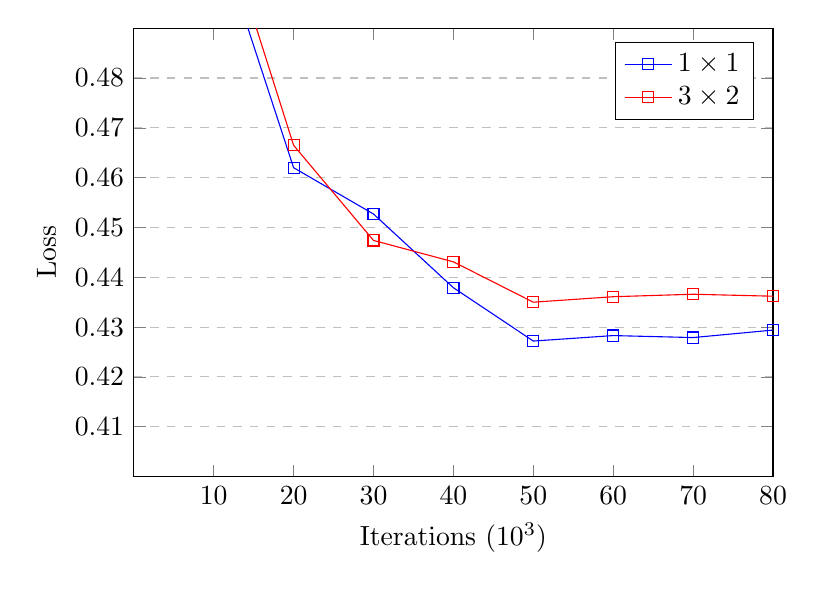
\begin{tikzpicture}
        \begin{axis}[
            width=0.8\textwidth,
            height=\axisdefaultheight,
            xlabel = {Iterations ($10^3$)},
            ylabel = {Loss},
            ymin = 0.40, ymax = 0.49, 
            xmin = 0, xmax = 80,
            xtick = {10, 20, 30, 40, 50, 60, 70, 80},
            ytick = {0.41, 0.42, 0.43, 0.44, 0.45, 0.46, 0.47, 0.48},
            ymajorgrids = true,
            yminorgrids = true,
            legend pos = north east,
            grid style = dashed
        ]
        \addplot[color=blue, mark=square]
            coordinates { (0,1)
            (10, 0.511)
            (20, 0.462)
            (30, 0.4527)
            (40, 0.4379)
            (50, 0.4272)
            (60, 0.4283)
            (70, 0.4279)
            (80, 0.4294)
            }; \addlegendentry{$1\times1$}        
    
        \addplot[color=red, mark=square]
            coordinates { (0,1)
            (10, 0.517)
            (20, 0.4665)
            (30, 0.4474)
            (40, 0.4431)
            (50, 0.435)
            (60, 0.4361)
            (70, 0.4366)
            (80, 0.4362)
            }; \addlegendentry{$3\times2$}
        \end{axis}
    \end{tikzpicture}
    \caption[Validation loss for two experiments applying both 
    a linear radius schedule and weight decay]
    {Validation loss for two experiments applying both 
    a linear radius schedule and weight decay with $\lambda = 0.05$ 
    using default hyperparameters.}
    \label{figure:final}
\end{figure}

\begin{figure}
    \centering
    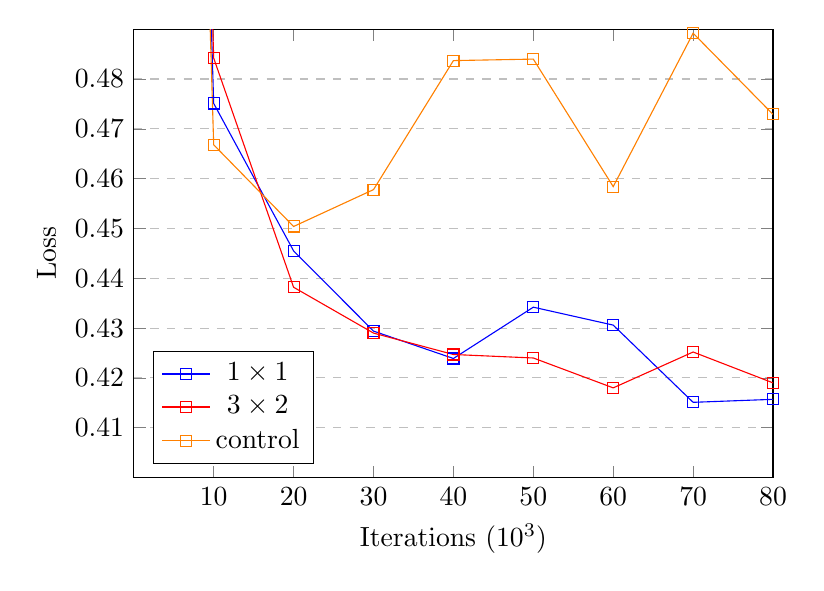
\begin{tikzpicture}
        \begin{axis}[
            width=0.8\textwidth,
            height=\axisdefaultheight,
            xlabel = {Iterations ($10^3$)},
            ylabel = {Loss},
            ymin = 0.40, ymax = 0.49, 
            xmin = 0, xmax = 80,
            xtick = {10, 20, 30, 40, 50, 60, 70, 80},
            ytick = {0.41, 0.42, 0.43, 0.44, 0.45, 0.46, 0.47, 0.48},
            ymajorgrids = true,
            yminorgrids = true,
            legend pos = south west,
            grid style = dashed
        ]
        \addplot[color=blue, mark=square]
        coordinates { (0,1)
        (10, 0.4751)
        (20, 0.4455)
        (30, 0.4294)
        (40, 0.4239)
        (50, 0.4342)
        (60, 0.4306)
        (70, 0.4151)
        (80, 0.4157)
        }; \addlegendentry{$1\times1$}        

    \addplot[color=red, mark=square]
        coordinates { (0,1)
        (10, 0.4842)
        (20, 0.4382)
        (30, 0.429)
        (40, 0.4247)
        (50, 0.424)
        (60, 0.418)
        (70, 0.4252)
        (80, 0.419)
        }; \addlegendentry{$3\times2$}

    \addplot[color=orange, mark=square]
        coordinates { (0,1)
        (10, 0.4668)
        (20, 0.4504)
        (30, 0.4578)
        (40, 0.4837)
        (50, 0.484)
        (60, 0.4584)
        (70, 0.4892)
        (80, 0.4729)
        }; \addlegendentry{control}
        \end{axis}
    \end{tikzpicture}
    \caption[Validation loss for two experiments applying both 
    a linear radius schedule and weight decay with a higher maximal radius]
    {Validation loss for two experiments applying both 
    a linear radius schedule and weight decay with $\lambda = 0.05$ 
    using a maximal radius of $R = 7.5 \cdot 10^{-3}$.
    The third control experiment uses the same $R$ but does not use
    a radius scheduler or weight decay.}
    \label{figure:final2}
\end{figure}

\begin{table}
    \centering
    \caption [Comparison of GLD and Adam in terms of 
    validation accuracy on SST-2 and memory consumption]
    {Comparison of GLD and Adam in terms of 
    validation accuracy on SST-2 and memory consumption.
    The Adam optimizer
    uses a learning rate of $5 \cdot 10^{-5}$ and a linear
    learning rate schedule. GLD methods set $K=5$ and
    $R = 5 \cdot 10^{-3}$. GLD* refers to our preferred 
    method, setting $R = 7.5 \cdot 10^{-3}$ while
    applying a linear radius schedule and 
    weight decay with $\lambda = 0.05$.
    Experiments with batch size 64
    run for $80,000$ steps, those with batch size 256 
    run for $40,000$ steps. Validation accuracy is 
    computed every $5,000$ steps.
    }
    \label{table:results}
    \bigskip
    \begin{tabular}{c c c c}
        \toprule
        \textbf{Optimizer} & \textbf{Batch Size} & \textbf{Validation Accuracy} & \textbf{Memory Consumption} \\
        \midrule
        GLD & 64 & 82.11\% & 409 MiB \\
        GLD* & 64 & 82.22\% & 409 MiB \\
        GLD & 256 & 84.17\% & 854 MiB \\
        Adam & 64 & 84.75\% & 421 MiB \\
        Adam & 256 & 84.40\% & 867 MiB \\
        \bottomrule
    \end{tabular}
\end{table}

